\documentclass[11pt, a4paper]{article}
\usepackage[utf8]{inputenc}
\usepackage[left=2cm, right=2cm, top=2.5cm, bottom=2.0cm]{geometry}
\usepackage{amsmath, amssymb, amsthm}
\usepackage[english]{babel}
\usepackage{graphicx}
\usepackage[font={small,it}]{caption}
\graphicspath{ {figures/} }
\usepackage{url}
\usepackage[toc,page]{appendix}
\usepackage{float}
\usepackage[bottom]{footmisc}
\usepackage{titling}
\usepackage[numbered,autolinebreaks,useliterate]{mcode}
%\setlength{\droptitle}{-10em}  

\title{ \huge Artificial Neural Networks \\ 
  { \large Project 2: Hopfield networks for character recognition}}
\author{
        Lood, Cédric \\
        \small Master of Bioinformatics
}

\begin{document}
\maketitle

\section{Context}
The analysis presented in this report was done for the class of
Artificial Neural Networks at KU Leuven (Spring 2016). It consists in
a practical implementation of a hopfield networks with the goal to
investigate retrieval capabilities of such networks for a given
digitized alphabet. The implementation was done in the MatLab
environment (2015a) using the neural networks toolbox. The scripts for
each of the sections can be found in the annex to this report.

\section{Hopfield network with 5 characters}

First we consider the creation of digital versions of characters. The
requirements were to build a sequence of characters (lowercase) using
our name + last name, followed by the uppercase alphabet. The
characters are represented by 7-by-5 matrices of 0s and 1s (0s being
interpreted as black, 1s as white). Figure \ref{fig:hopfield_chargen}
illustrates a sequence of such characters.

\begin{figure}[H]
  \centering
  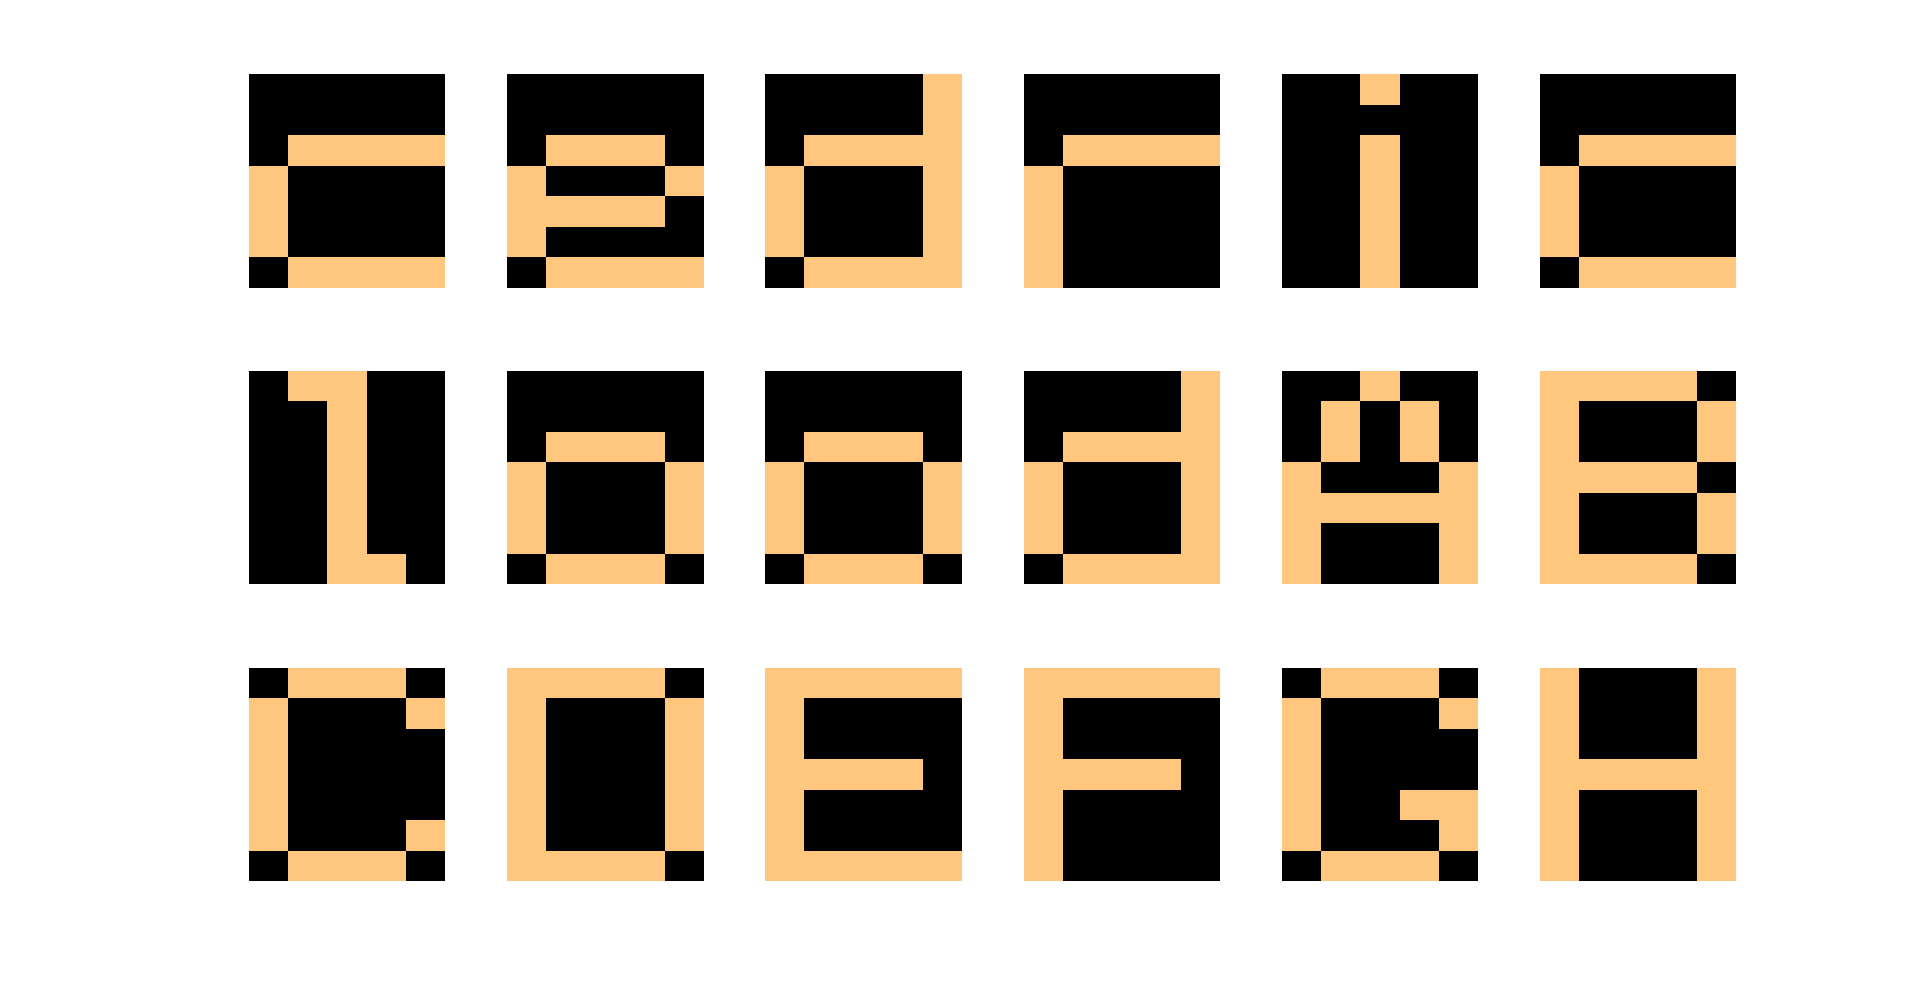
\includegraphics[scale=.30]{hopfield_chargen.png}
  \caption{Partial character sequence dataset}
  \label{fig:hopfield_chargen}
\end{figure}

An hopfield network was then created to store the first 5 letters of
the sequence as attractor points. One of the thing to keep in mind in
doing so is that the patterns that the hopfield net can store consists
of -1s and 1s, instead of 0s and 1s, so first a conversion needs to be
done. 

To test the retrieval of the points, some noise was added by flipping
3 random positions in the character, then presenting them to the
network to see if they could be retrieved. This process is illustrated
on figure \ref{fig:hopfield_chargen}

\begin{figure}[H]
  \centering
  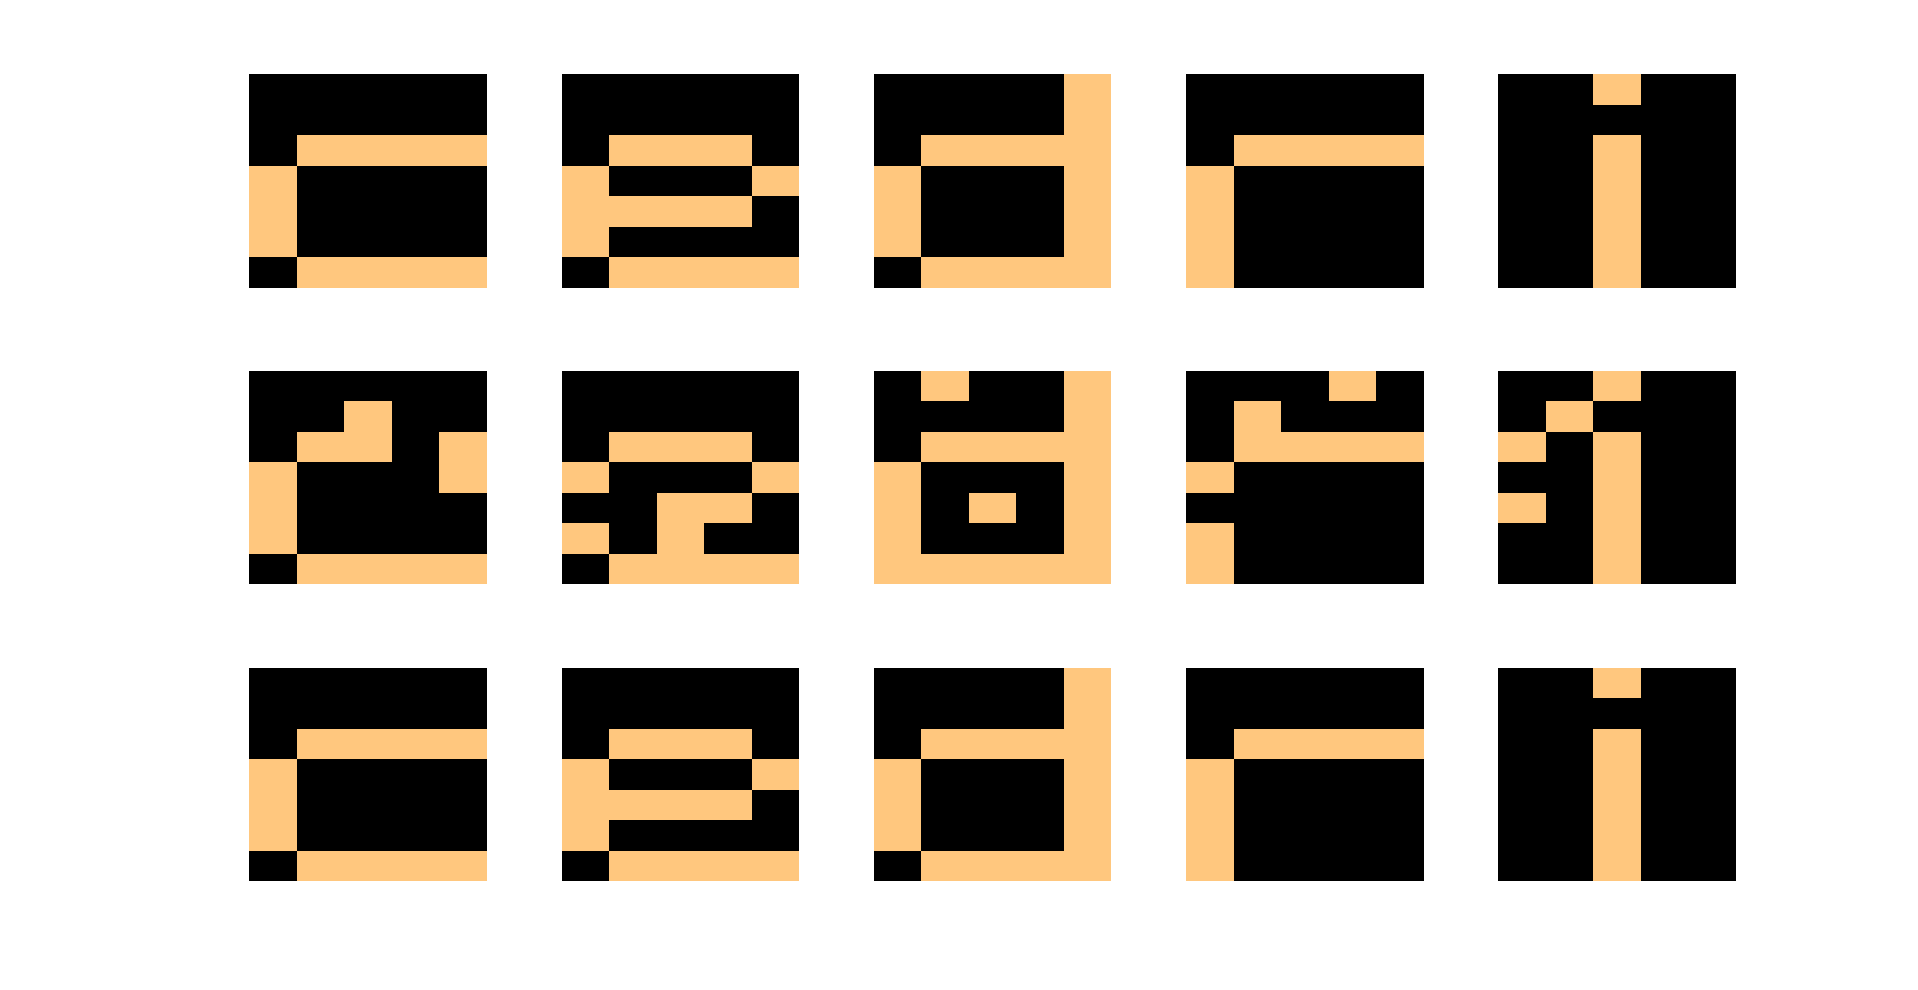
\includegraphics[scale=.30]{hopfield_denoising.png}
  \caption{Top: original letters, middle: added noise, bottom:
    retrieval from hopnet}
  \label{fig:hopfield_chargen}
\end{figure}

While the process above did work perfectly, it is not immune to
spurious states. Those are states that are not explicitely put into
the network as attractors when it is build. As mentioned in the matlab
manual for Hopfield networks, the design method guarantees the
existence of the attractors explicitely put into the network, but the
existence of other attractors is not excluded.

\section{Critical loading capacity}

I started by looking how far I could push the network before I would
start seeing spurious state appear visually by plotting the
reconstructed characters. From 16 characters, I started obtaining some
spurious states by varying multiple reconstructions of stochastic
noisy characters (ie, for multiple random seeds). Figure
\ref{fig:hopfield_rnd7} shows a perfect reconstruction of the 16
characters for a random seed of 7, while for the same configuration,
but with a random seed of 8, we observe (figure
\ref{fig:hopfield_rnd8}) spurious states, interestingly we also
observe a mis-reconstructed ``l'' instead of the original ``i''. This
can be understood given the closeness of both characters.

\begin{figure}[H]
  \centering
  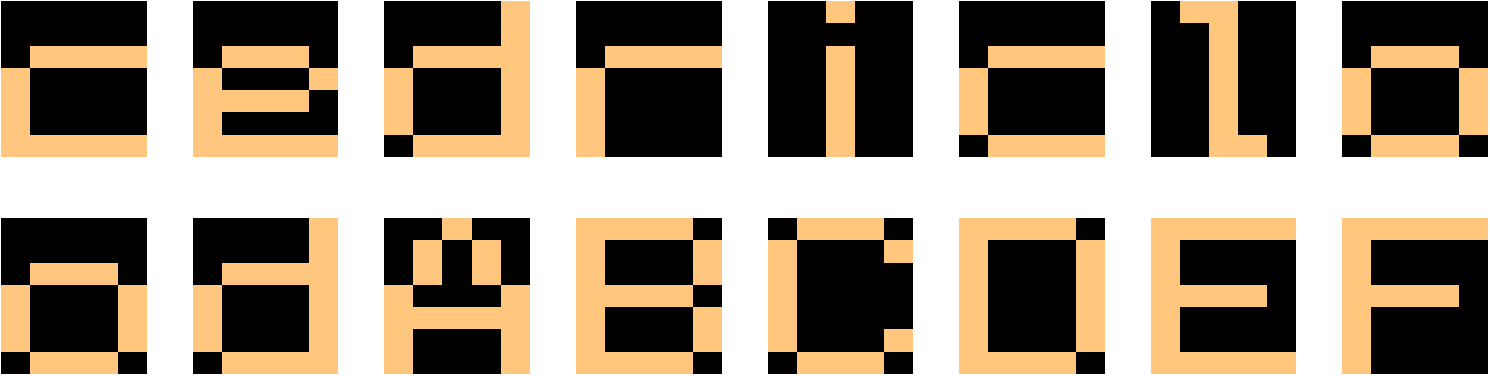
\includegraphics[scale=.30]{hopfield_spurious_rnd7.png}
  \caption{Perfect reconstruction of 16 characters}
  \label{fig:hopfield_rnd7}
\end{figure}

\begin{figure}[H]
  \centering
  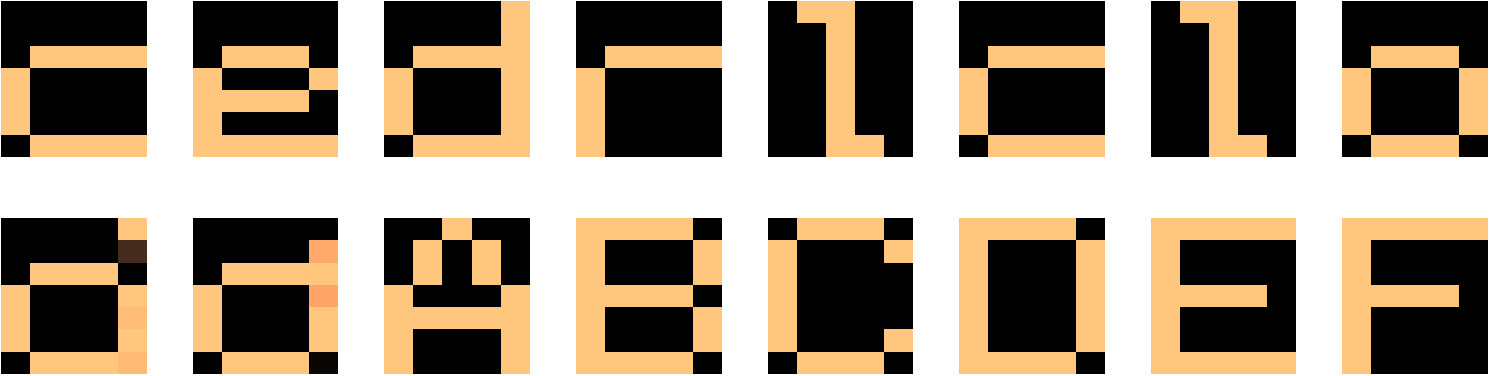
\includegraphics[scale=.30]{hopfield_spurious_rnd8.png}
  \caption{Same configuration as above (different noise), imperfect reconstruction}
  \label{fig:hopfield_rnd8}
\end{figure}

Given the variation in the results for different initialization, I
proceeded to evaluate the reconstructions errors as indicated in the
instructions over 50 different values of random seeds. The results are
reported in figure \ref{fig:hopfield_error}

\begin{figure}[H]
  \centering
  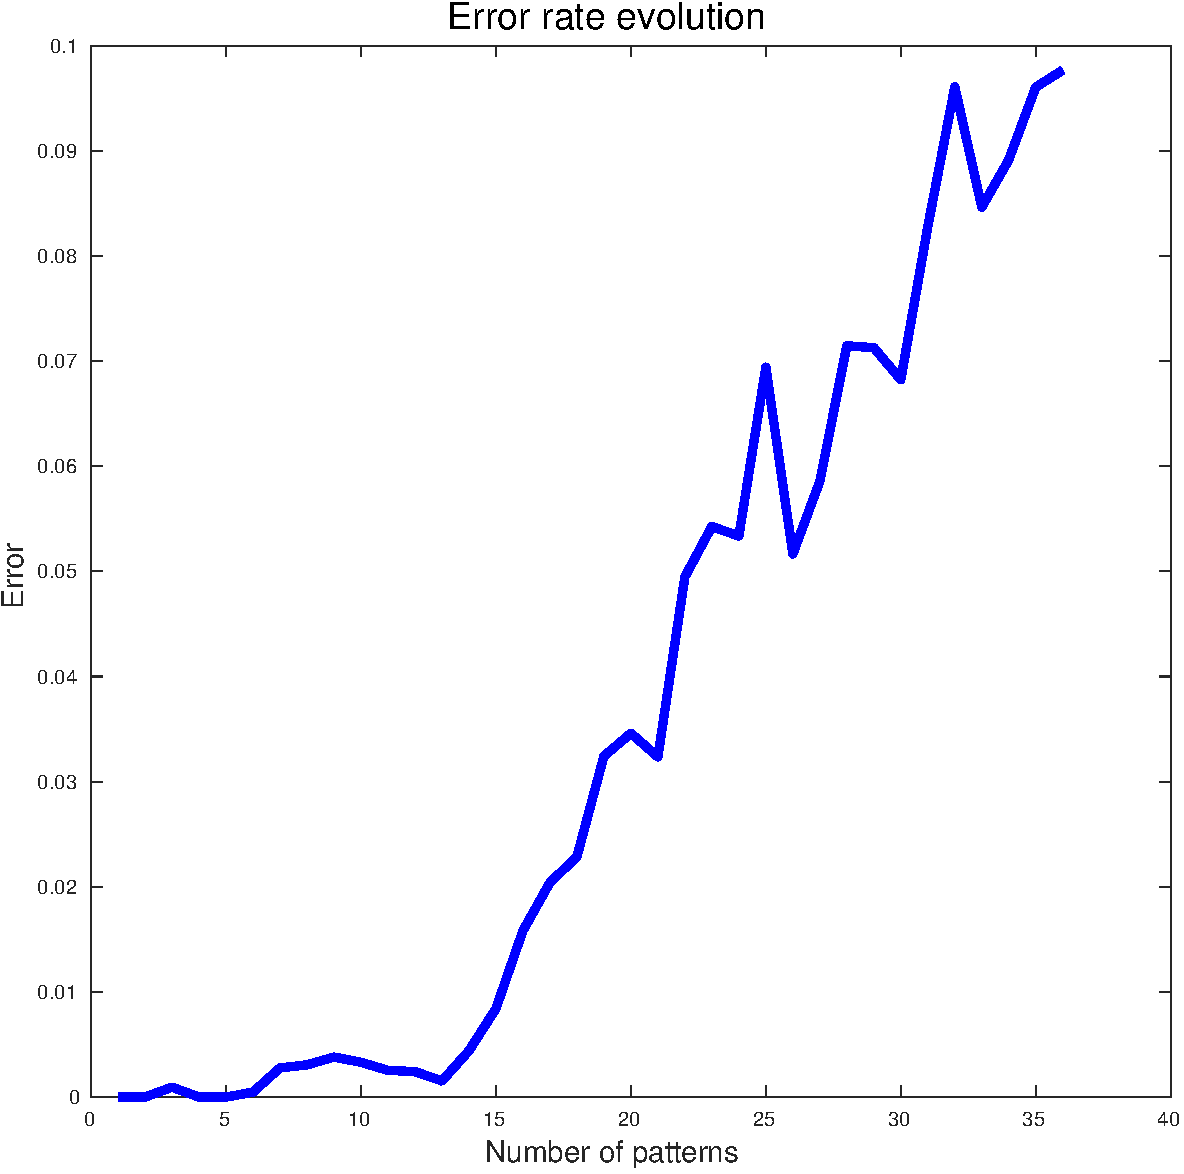
\includegraphics[scale=.50]{hopfield_error.pdf}
  \caption{Reconstruction error for increasing number of stored patterns}
  \label{fig:hopfield_error}
\end{figure}

In total we use 35 neurons to store 36 different patterns, so it is
easy to calculate the theoritical storage capacity for perfect
retrieval, which is expressed mathematically by
$p_{max}=\frac{N}{4logN}=2.46$. The error graph seems to validate this
estimation, as there is indeed not a single error over the 50
reconstructions for less than 3 patterns.

\section{Perfect retrieval of character set}

In order to achieve perfect retrieval, a technique that would
certainly work is to increase the number of neurons available in the
network. The number of patterns would stay fixed at 36. To determine
the number of neurons required, we could try to switch the storage
capacity formula and solve for $N$, but that is not trivial. In fact,
we need to approximate the solution to this equation (using for
example Lambert W
function\footnote{https://en.wikipedia.org/wiki/Lambert\_W\_function}). I
used a numerical method to estimate the value of N, and found that for
$N=160$ we would be able to store all patterns without errors.

One way to proceed then, is simply to scale up the numbers of pixels
by boosting the density artificially. By replacing each pixels by
3-by-3 pixels of the same value, one easily reaches the number of
neurons necessary for perfect retrieval. Doing so using the same
dataset resulted in no errors.

\begin{appendices}
\section{Hopnet}
\subsection{Part 1}
\begin{lstlisting}
clc, clear all, close all;
addpath 'export_fig'; % export pdf: https://github.com/altmany/export_fig
rng(7); % setting random seed

% generating data
%%%%%%%%%%%%%%%%%
characters = character_generator();
figure('Color', [1 1 1]);
for i = 1:18
    subplot(3,6,i);
    imagesc(reshape(characters(:,i),5,7)',[0,1]);
    axis off; colormap copper;
end

export_fig('hopfield_chargen.pdf');

% trick to rescal to -1 1 instead of 0 1 (requirement hopfield)
characters = 2*characters -1;

% Training network
%%%%%%%%%%%%%%%%%%
net = newhop(characters(:,1:5));

% plot original first 5 letters
figure('Color', [1 1 1]);
for i = 1:5
    subplot(3,5,i);
    imagesc(reshape(characters(:,i),5,7)',[0,1]);
    axis off; colormap copper;
end

% plot first 5 letters with noise
noisy_digits = zeros(35,5);
for i=1:5
    noisy_digits(:,i)=noise3(characters(:,i));
end
noisy_digits_plot = (noisy_digits+1)/2;
for i = 1:5
    subplot(3,5,i+5);
    imagesc(reshape(noisy_digits_plot(:,i),5,7)',[0,1]);
    axis off; colormap copper;
end

% reconstitute letters
for i = 1:5
    [Y Pf Af] = sim(net, {1 10}, [], {noisy_digits(:,i)});
    C = Y{1,10};
    recon_digits_plot = (C+1)/2;
    subplot(3,5,i+10);
    imagesc(reshape(recon_digits_plot(:,1),5,7)',[0,1]);
    axis off; colormap copper;
end

% Critical loading of network
%%%%%%%%%%%%%%%%%%%%%%%%%%%%%
n_rand = 50;
errors = zeros(36, n_rand);

for randg = 1:n_rand % loop over 10 different seeds
    rng(randg);
    %errors = zeros(36, 1);
    for p = 1:36 % loop over a total number of 36 characters
        net = newhop(characters(:,1:p));
        reconstructed_chars = zeros(35, p);
        noisy_digits = zeros(35,p);
        
        for i=1:p % addition of noise
            noisy_digits(:,i)=noise3(characters(:,i));
        end
    
        for i=1:p % reconstruction
            [Y Pf Af] = sim(net, {1 100}, [], {noisy_digits(:,i)});
            reconstructed_chars(:,i) = Y{1,100};
        end
        errors(p, randg) = sum(sum(reconstructed_chars ~= characters(:,1:p)));
    end
end

% averaging errors over multiple random seeds
frac_errors = zeros(36,1);
for p=1:36
    frac_errors(p) = sum(errors(p,:))/n_rand
    frac_errors(p) = frac_errors(p)/(p*35);
end

figure('Color', [1 1 1]);
plot(1:36, frac_errors, 'b-','linewidth',4);
title('Error rate evolution','FontSize',18,'FontWeight', 'normal');
xlabel('Number of patterns','FontSize',14);
ylabel('Error','FontSize',14);

% theoritical capacity
disp(35/(4*log(35)));

res=0;
for i=1:500
    res = exp(i)/i;
    if(res > 10e+66)
        disp(i);
        break;
    end
    disp(res);
end

% Perfect retrieval
%%%%%%%%%%%%%%%%%%%
dense_char = zeros(35*9, 36);
for i=1:36
    position = 1;
    for j=1:35*9
        dense_char(j,i) = characters(position, i);
        if(~mod(j, 9))
            position = position + 1;
        end
    end
end

net = newhop(dense_char(:,1:36));
noisy_digits = zeros(35*9,36);

for i=1:36 % addition of noise
    noisy_digits(:,i)=noise3(dense_char(:,i));
end
for i=1:36 % reconstruction
    [Y Pf Af] = sim(net, {1 100}, [], {noisy_digits(:,i)});
    reconstructed_chars(:,i) = Y{1,100};
end

errors = sum(sum(reconstructed_chars ~= dense_char));

\end{lstlisting}
\subsection{Helper functions: character generator}
\begin{lstlisting}
function [characters] = character_generator()
c = [ 
    0 0 0 0 0 ...
    0 0 0 0 0 ...
    0 1 1 1 1 ...
    1 0 0 0 0 ...
    1 0 0 0 0 ...
    1 0 0 0 0 ...
    0 1 1 1 1 ]';
e = [
    0 0 0 0 0 ...
    0 0 0 0 0 ...
    0 1 1 1 0 ...
    1 0 0 0 1 ...
    1 1 1 1 0 ...
    1 0 0 0 0 ...
    0 1 1 1 1 ]';
d = [
    0 0 0 0 1 ...
    0 0 0 0 1 ...
    0 1 1 1 1 ...
    1 0 0 0 1 ...
    1 0 0 0 1 ...
    1 0 0 0 1 ...
    0 1 1 1 1 ]';
r = [ 
    0 0 0 0 0 ...
    0 0 0 0 0 ...
    0 1 1 1 1 ...
    1 0 0 0 0 ...
    1 0 0 0 0 ...
    1 0 0 0 0 ...
    1 0 0 0 0 ]';
i = [
    0 0 1 0 0 ...
    0 0 0 0 0 ...
    0 0 1 0 0 ...
    0 0 1 0 0 ...
    0 0 1 0 0 ...
    0 0 1 0 0 ...
    0 0 1 0 0 ]';
l = [
    0 1 1 0 0 ...
    0 0 1 0 0 ...
    0 0 1 0 0 ...
    0 0 1 0 0 ...
    0 0 1 0 0 ...
    0 0 1 0 0 ...
    0 0 1 1 0 ]';
o = [
    0 0 0 0 0 ...
    0 0 0 0 0 ...
    0 1 1 1 0 ...
    1 0 0 0 1 ...
    1 0 0 0 1 ...
    1 0 0 0 1 ...
    0 1 1 1 0 ]';   
characters = [c, e, d, r, i, c, l, o, o, d, prprob];
\end{lstlisting}
\subsection{Helper function: noise3}
\begin{lstlisting}
function [noisy_digit] = noise3(digit)
noisy_digit = digit;
[m, n] = size(digit);
noise = randperm(m);
noise = noise(1:3); % selects 3 positions to flip
for i=1:3
    noisy_digit(noise(i)) = -noisy_digit(noise(i));
end
\end{lstlisting}
\end{appendices}
\end{document}
